\newsavebox{\sonorityanglehierarchycompressed}
\savebox{\sonorityanglehierarchycompressed}{
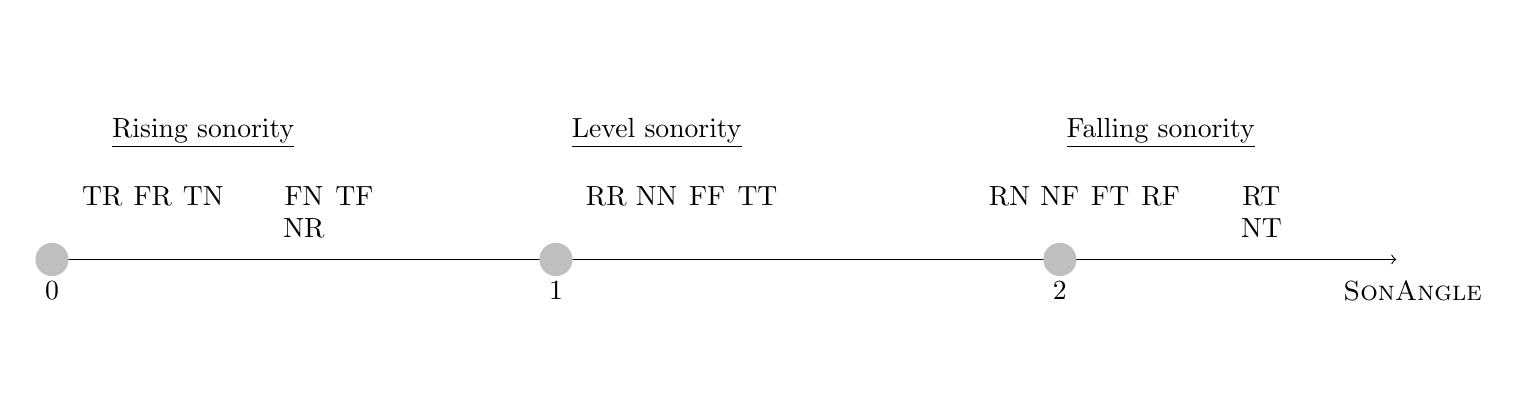
\begin{tikzpicture}[scale=0.8,shorten >=1pt,->]
  \tikzstyle{vertex}=[circle]
  \tikzstyle{point}=[circle,fill=black!25,minimum size=12pt,inner sep=2pt]
  \tikzstyle{line} = [draw, -latex']
  \node[vertex] (RT) at (2.4*8,1)   {RT};
  \node[vertex] (NT) at (2.4*8,0.5)  {NT};
  \node[vertex] (FT) at (2.1*8,1)  {FT};
  \node[vertex] (TT) at (1.4*8,1)     {TT};
  \node[vertex] (RF) at (2.2*8,1)     {RF};
  \node[vertex] (NF) at (2.0*8,1)  {NF};
  \node[vertex] (TF) at (0.6*8,1)   {TF};
  \node[vertex] (FF) at (1.3*8,1)   {FF};
  \node[vertex] (RN) at (1.9*8,1)   {RN};
  \node[vertex] (NN) at (1.2*8,1)   {NN};
  \node[vertex] (FN) at (0.5*8,1)  {FN};
  \node[vertex] (TN) at (0.3*8,1)   {TN};
  \node[vertex] (RR) at (1.1*8,1)  {RR};
  \node[vertex] (NR) at (0.5*8,0.5)  {NR};
  \node[vertex] (FR) at (0.2*8,1)   {FR};
  \node[vertex] (TR) at (0.1*8,1)   {TR};
  \node[vertex] (rising) at (0.3*8,2) {\underline{Rising sonority}};
  \node[vertex] (level) at (1.2*8,2) {\underline{Level sonority}};
  \node[vertex] (falling) at (2.2*8,2) {\underline{Falling sonority}};
  % axis
  \node[vertex] (axisstart) at (0.0,0) {};
  \node[vertex] (axisend)   at (2.7*8,0) {};
  \draw (axisstart) -- (axisend);
  \node[point]  (0point) at (0.0,0) {};
  \node[point]  (1point) at (1.0*8,0) {};
  \node[point]  (2point) at (2.0*8,0) {};
  \node[vertex] (0pointlabel) at (0.0,-0.5) {0};
  \node[vertex] (1pointlabel) at (1.0*8,-0.5) {1};
  \node[vertex] (2pointlabel) at (2.0*8,-0.5) {2};
  \node[vertex] (xaxislabel) at (2.7*8,-0.5) {\textsc{SonAngle}};
\end{tikzpicture}
}


